\documentclass[10pt]{article}

% required packages
\usepackage{graphicx}
\usepackage{subfigure} 
\usepackage[hidelinks]{hyperref}
\usepackage{fancyhdr}

% better tables
\usepackage{booktabs}
\usepackage{multirow}
\newcommand{\ra}[1]{\renewcommand{\arraystretch}{#1}}

% margins
\setlength{\headwidth}{6.40in}
\pagestyle{fancy}
\addtolength{\textwidth}{1in}
\addtolength{\textheight}{1in}
\addtolength{\evensidemargin}{0.5in}
\addtolength{\oddsidemargin}{-0.5in}
\addtolength{\topmargin}{-0.5in}


% page headers
\fancyhead{} 
\fancyhead[LO,LE]{CSE 250B}
\fancyhead[RO,RE]{Project 3}


\title{Topic Classification using Latent Dirichlet Allocation}

\author{Adrian Guthals (aguthals@cs.ucsd.edu),\\
David Larson (dplarson@ucsd.edu),\\
\\
CSE 250B: Project \#3 \\
University of California, San Diego \\
}


\begin{document}

\maketitle


%-----------------------------------------------------------------------------
% ABSTRACT
%-----------------------------------------------------------------------------
\begin{abstract}
LDA, Gibbs sampling, topic classification of documents, datasets used, results and their meaning, conclusions
\end{abstract}



%-----------------------------------------------------------------------------
% INTRODUCTION
%-----------------------------------------------------------------------------
\section{Introduction}
\label{sec:intro}

Introduce topic classification of documents. Then transition into formal definitions of LDA and Gibbs Sampling.

Elkan's lecture notes \cite{CSE250B}


\subsection{Latent Dirichlet Allocation}
\label{sec:lda}

Latent Dirichlet Allocation (LDA) is a multinomial

\begin{equation}
    p(\gamma | \alpha) = \frac{1}{D(\alpha)} \prod_{s=1}^{m} \gamma_{s}^{\alpha_s - 1}
\end{equation}

\begin{equation}
    D(\alpha) = \int_{\gamma} \prod_{s=1}^m \gamma_s^{\alpha_s - 1}
\end{equation}

\begin{equation}
    D(\alpha) = \frac{\prod_{s=1}^m \Gamma(\alpha_s)}{\Gamma (\sum_{s=1}^m \alpha_s )}
\end{equation}



\subsection{Gibbs Sampling}
\label{sec:gibbs}

\begin{equation}
    p(z_i = j | \bar{z}', \bar{w}) \propto \frac{q_{j w_i}' + \beta_{w_i}}{\sum_t q_{jt}' + \beta_t} \frac{n_{mj}' + \alpha_j}{\sum_k n_{mk}' + \alpha_k}
\end{equation}



%-----------------------------------------------------------------------------
% ALGORITHMS
%-----------------------------------------------------------------------------
\section{Design and Analysis of Algorithms}
\label{sec:algorithms}

We implemented the LDA generative process as outlined in \cite{CSE250B}.

Discuss how we're implementing LDA and Gibbs Sampling.



%-----------------------------------------------------------------------------
% EXPERIMENTS
%-----------------------------------------------------------------------------
\section{Design of Experiments}
\label{sec:experiments}

%
% DATASETS
%
\subsection{Datasets}
Two datasets were classified using LDA: Classic400, a collection of English documents from three research areas (aeronautics, medicine, and library science); and KOS, a collection of English blog posts from dailykos.com (see Table \ref{tab:datasets} for details on their sizes) \cite{Classic400, KOS_dataset}. While the Classic400 dataset provided the true labels of its source topics, the KOS dataset provided no such information. Also, to reduce run times, we elected to use a reduced version of the KOS dataset containing only the first 400 of the original 3430 documents.


\begin{table}[t]
    \centering
    \ra{1.2}
    \begin{tabular}{@{} l l l l l @{}}
        \toprule
        \bf{Dataset} & \bf{Documents} & \bf{Vocabulary} & $\alpha$ & $\beta$ \\
        \midrule
        Classic400 & 400 & 6205 & 0.01 & 0.1 \\
        KOS        & 400 & 6906 & 0.01 & 0.1\\
        \bottomrule
    \end{tabular}
    \caption{Composition of the two datasets used in this study and the chosen Gibbs hyperparameters $\alpha$ and $\beta$. Note that the KOS dataset used is a reduced version of the original KOS dataset, which contains 3430 documents.}
    \label{tab:datasets}
\end{table}


%
% HYPERPARAMETERS
%
\subsection{Hyperparameters}
For both datasets we apply LDA with three topics ($K = 3$). Since $\alpha$ is postively correlated to the number of topics present per document and we are only considering three topics, we chose values of $\alpha << 1$, which implies that every document contains only a few topics. Likewise, we chose values of $\beta << 1$, which implies that every word in every document corresponds to a small number of topics. Previous studies have looked into the effect of $\alpha$ and $\beta$ on the cluserting results for LDA models, some going so far as to suggest likely values based on the number of topics in a dataset (see \cite{Griffiths2004}). 


However, for the purposes of this study our selection criteria of $\alpha$ and $\beta$ is only that they are both small, and we have therefore chosen to use a grid search method to determine the optimal values. We ran trained the LDA model using Gibbs sampling for $\alpha$ and $\beta$ values of $10^2, 10^1, ..., 10^{-4}$, and evaluated the values based on the coherence of each topics' most commonly occurred words. From this grid search we chosen to set $\alpha = 0.01$ and $\beta = 0.1$ for both datasets (see Table \ref{tab:datasets}).


%
% CONVERGENCE
%
\subsection{Stopping Criteria of Gibbs Sampling}
For both datasets we chose the Gibbs Sampling stopping criteria as 100 epochs. We tried 50, 75, ..., 200 epochs as the stopping criteria, but found that the Euclidean distance between the $\phi$ vectors to not change signifcantly for more than 100 epochs.

%
% OVERFITTING
%
\subsection{Overfitting}
As with many models, LDA is susceptible to overfitting. One approach to determine overfitting of a LDA model is to calculate the perplexity of the model (see \cite{Heinrich}).


%
% RESULTS
%
\subsection{Results}

\subsubsection{Document Topic Clustering}
Figure \ref{fig:cluserting} shows the clustering of documents relative to each topic as projected onto a triangular simplex, where the each vertex indicates $\theta = 1$ for the denoted topic.


\begin{figure}[t]
    \centering
    \mbox{\subfigure[Classic400]{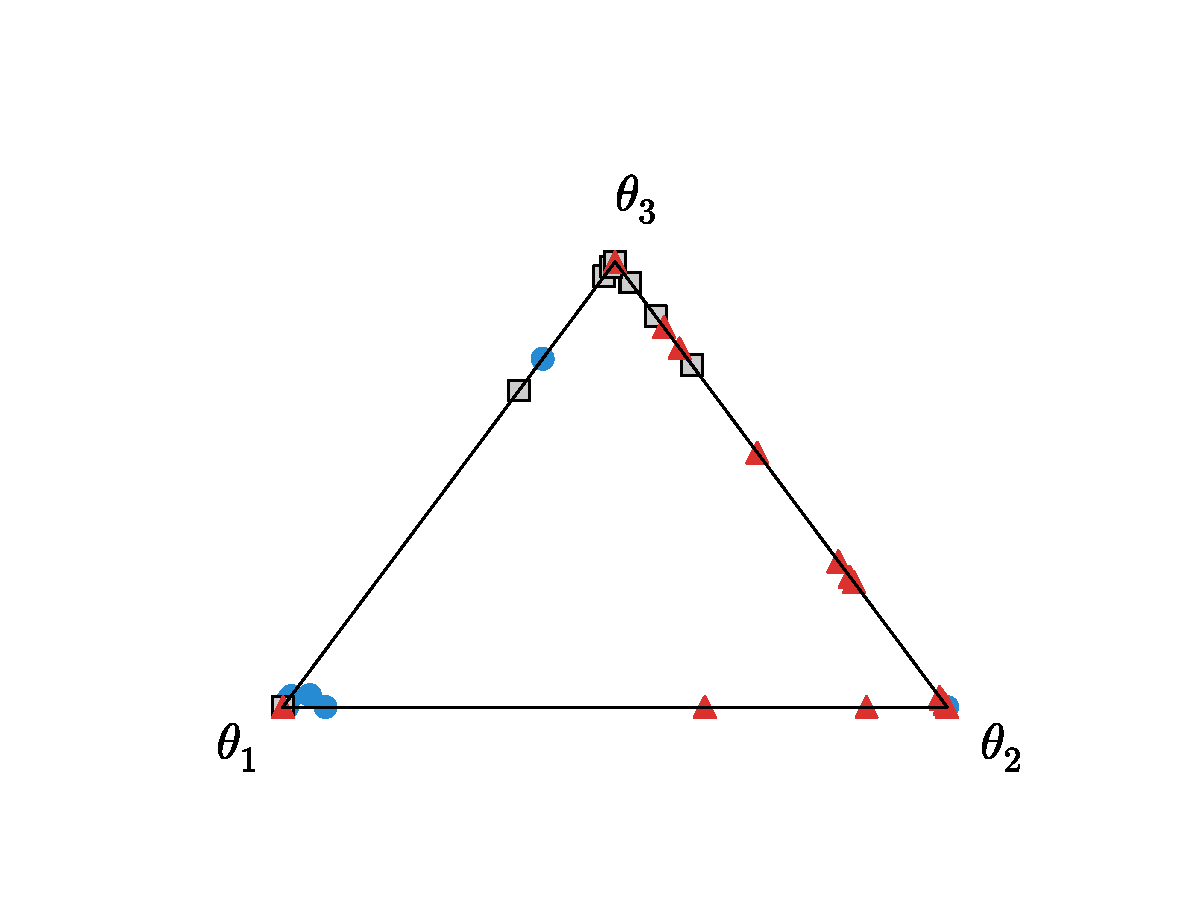
\includegraphics[width=0.5\textwidth]{classic400_thetas.pdf}} \quad
        \subfigure[KOS]{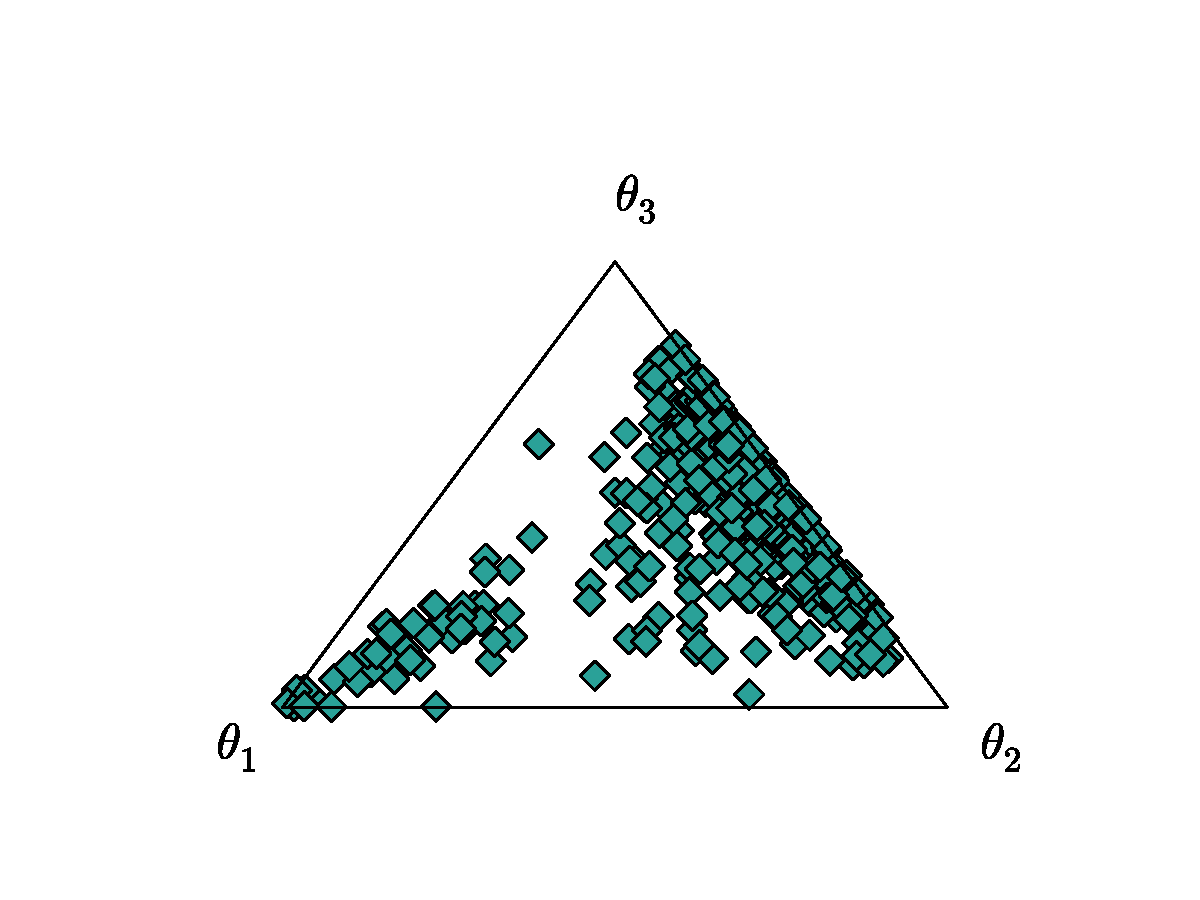
\includegraphics[width=0.5\textwidth]{kos_thetas.pdf} }}
    \caption{Clustering of documents based on their $\theta_1$, $\theta_2$ and $\theta_3$, projected on a triangular simplex. Documents in Classic400 are labeled based on their true labels (topic 1: white circles with black edges, topic 2: black solid squares, topic 3: gray solid triangles) while documents in KOS are have the same marker label as the true labels are unknown.}
    \label{fig:cluserting}
\end{figure}


\subsubsection{Most Common Words Per Topic}
If a LDA model is setup to classify more than 4 topics, then a simplex plot will not be a viable method for checking the clustering of the results. Instead, lists of the most commonly occurred words per topic can be analyzed to gauge the performance of the LDA. Table \ref{tab:most_common} shows the most commonly occurred words for each topic of the two datasets. The most common words from Classic400 for each topic are all related and correspond well to the true topic labels (topic 1: medicine, topic 2: aeronautics, and topic 3: library science). Meanwhile, the most common words for KOS for each topic seem to overlap and be derived from same general topic, namely politics, or more specifically, the 2008 US Presidential campaign between George Bush and John Kerry. As the source of KOS is a political blog site, it is not surprising that politics shows up prominetly as a topic. However, the lack of diversity between the most common words of each topic and therefore lack of unique topics is more likely the result of selecting only the first 400 documents from the originald dataset rather than an issue with our LDA model implementation.



\begin{table}[t]
	\centering
    \ra{1.2}
	\begin{tabular}{@{} l l l l c l l l @{}}
        \toprule
        & \multicolumn{3}{c}{Classic400} & \phantom{abc} & \multicolumn{3}{c}{KOS}\\
        \cmidrule{2-4} \cmidrule{6-8}
        \bf{Rank} & \bf{Topic 1} & \bf{Topic 2} & \bf{Topic 3} && \bf{Topic 1} & \bf{Topic 2} & \bf{Topic 3} \\
        \midrule
         1 & system     & boundary      & patients      && bush             & republican    & november \\
         2 & research   & layer         & ventricular   && kerry            & race          & kerry \\
         3 & scientific & wing          & fatty         && war              & house         & voting \\
         4 & retrieval  & mach          & cases         && iraq             & party         & vote \\
         5 & problems   & supersonic    & nickels       && people           & elections     & bush \\
         6 & language   & wings         & left          && president        & campaign      & polls \\
         7 & science    & ratio         & acids         && general          & democratic    & poll \\
         8 & methods    & velocity      & aortic        && voters           & state         & governor \\ 
         9 & systems    & effects       & blood         && administration   & democrats     & senate \\
        10 & subject    & shocks        & normal        && time             & senate        & republicans \\
        \bottomrule
	\end{tabular}
	\caption{Ten most commonly occured words for each topic classification for the classic400 and KOS datasets. Rank indicates how frequently a word appears in each topic, with 1 being the most occurred.}
	\label{tab:most_common}
\end{table}



%-----------------------------------------------------------------------------
% CONCLUSION
%-----------------------------------------------------------------------------
\section{Findings and Lessons Learned}
\label{sec:conclusion}

Thoughts on: LDA as a model, Gibbs Sampling as a training method, performance issues, results of the experiments


%-----------------------------------------------------------------------------
% BIBLIOGRAPHY
%-----------------------------------------------------------------------------
\bibliographystyle{IEEEtran}
\bibliography{sources}


\end{document}
